
\bigskip


\noindent
\underline{$e^- e^- \to e^- e^-$ (M{\o}ller scattering)}\\
Initial and final states:
\begin{eqnarray}
\begin{array}{l}
\ketend i \ket
= c_{r_a}^\dagger (\bld{p}_a) c_{r_b}^\dagger (\bld{p}_b) \ketend 0 \ket
\rightdef \ketend e^-_a, e^-_b \ket
\vspace{2mm}
\\
\ketend f \ket
= c_{r_1}^\dagger (\bld{p}_1) c_{r_2}^\dagger (\bld{p}_2) \ketend 0 \ket
\rightdef \ketend e^-_1, e^-_2 \ket
\end{array}
\end{eqnarray}
We use notations used in \ref{sec:DiracYukawa} to write
the second order S-matrix as
\begin{eqnarray}
\bra f \braend S^{(2)} \ketend i \ket
&=&
\frac{(-i)^2}{2}
\int d^4 x_{1'} d^4 x_{2'}
\;\bra f \braend T[ {\cal H}_{int}(x_1') {\cal H}_{int}(x_2')] \ketend i \ket
\nonumber\\
&=&
\frac{(-ie)^2}{2}
\int d^4 x_1' d^4 x_2'
\nonumber\\
&&
<e^-_2, e^-_1 \braend T \left[
\normalprod{
\overline{\psi}_{1'}
\slashed{A}_{1'} \psi_{1'}
}
\normalprod{
\overline{\psi}_{2'}
\slashed{A}_{2'} \psi_{2'}
}
\right]
\ketend e^-_a e^-_b \ket
\nonumber\\
&=&
\frac{(-ie)^2}{2}
\int d^4 x_{1'} d^4 x_{2'}
\bra 0 \braend T\left[
A_{1'}^\mu A_{2'}^\nu
\right] \ketend 0 \ket
\nonumber\\
&&
<e^-_2, e^-_1 \braend T \left[
\normalprod{
\overline{\psi}_{1'}
\gamma_\mu \psi_{1'}
}
\normalprod{
\overline{\psi}_{2'}
\gamma_\nu \psi_{2'}
}
\right]
\ketend e^-_a e^-_b \ket
\nonumber\\
&=&
\frac{(-ie)^2}{2}
\int d^4 x_{1'} d^4 x_{2'}
D_F^{\mu \nu}(x_{1'} - x_{2'}) 
(\gamma_\mu)_{\alpha \beta}
(\gamma_\nu)_{\gamma \delta} 
\nonumber\\
&&
<e^-_2, e^-_1 \braend T \left[
\normalprod{
\overline{\psi}_{1' \alpha}
 \psi_{1' \beta}
}
\normalprod{
\overline{\psi}_{2' \gamma}
\psi_{2' \delta}
}
\right]
\ketend e^-_a e^-_b \ket
\nonumber\\
\label{eqn:SmatrixMoller1}
\end{eqnarray}
%-----------------------------------------------
\begin{eqnarray}
&&
<e^-_2, e^-_1 \braend T \left[
\normalprod{
\overline{\psi}_{1' \alpha}
 \psi_{1' \beta}
}
\normalprod{
\overline{\psi}_{2' \gamma}
\psi_{2' \delta}
}
\right]
\ketend e^-_a e^-_b \ket
\nonumber\\
&& 
=
<e^-_2, e^-_1 \braend 
\normalprod{
\overline{\psi^{(+)}_{1' \alpha}}
\, \psi^{(+)}_{1' \beta}
\,\overline{\psi^{(+)}_{2' \gamma}}
\,\psi^{(+)}_{2' \delta}
}
\ketend e^-_a e^-_b \ket
\nonumber\\
&& 
=
<e^-_2, e^-_1 \braend 
\overline{\psi^{(+)}_{1' \alpha}}
\,\overline{\psi^{(+)}_{2' \gamma}}
\,\psi^{(+)}_{2' \delta}
\, \psi^{(+)}_{1' \beta}
\ketend e^-_a e^-_b \ket
\nonumber\\
&& 
=
< 0 \braend c_2 c_1
\left\{
c^\dagger_{1' (1')} c^\dagger_{2' (2')}
c_{2' (b')} c_{1' (a')}
\right\}
c_a^\dagger c_b^\dagger \ketend 0 \ket
%\nonumber\\
%&&
\bar{u}_\alpha^{(1')} \bar{u}_\gamma^{(2')}
u_\delta^{(b')} u_\beta^{(a')}
\nonumber\\
\label{eqn:Mollerambabbr}
\end{eqnarray}
The last expression can be compared with Eq. (\ref{eqn:DirNNNNsandIntermed}).
Proceeding further we obtain an expression quite similar with Eq. (\ref{eqn:DirNNNNabbamp}):
\begin{eqnarray}
(\ref{eqn:Mollerambabbr}) 
&=&
\frac{1}{(2\pi)^6}
\sum_{(1')(2')(a')(b')}
\left\{
(
\delta_{(1')1}\delta_{(2')2}
-
\delta_{2(1')}\delta_{1(2')}
)
(
\delta_{(a')a}\delta_{(b')b}
-
\delta_{(a')b}\delta_{(b')a}
)
\right\}
 \times
\nonumber\\
&&
e^{i(p_{1'} x_{1'} + p_{2'} x_{2'}  - p_{a'} x_{1'} - p_{b'} x_{2'}    )}
\bar{u}_\alpha^{(1')} u_\beta^{(a')} \bar{u}_\gamma^{(2')} u_\delta^{(b')}
\label{eqn:Mollerabbamp2}
\end{eqnarray}
In \ref{sec:DiracYukawa}, we have made use of a fact that boson propagator $\Delta_F(x)$ is an
even function. $D_F^{\mu \nu} (x)$ in Eq. (\ref{eqn:SmatrixMoller1}) is also even and symmetric 
about suffices $\mu$ and $\nu$ as it is observed in Eq. (\ref{eqn:photonPropalpha}).
Setting $\alpha = 1$ 
%as is mentioned before
, we have
\begin{eqnarray}
S_{fi}^{(2)}
&=&
\frac{(-ie)^2}{(2\pi)^6}
\int d^4 k
\frac{-ig^{\mu \nu }(2\pi)^4}{k^2 + \i\epsilon}
\nonumber\\
&&
\hspace{10mm}
\left\{
\delta^4(p_1 - p_a - k) \delta^4(p_2 - p_b + k)
\left[\bar{u}^{(1)} \gamma_\mu u^{(a)} \right]
\left[ \bar{u}^{(2)} \gamma_\nu u^{(b)} \right]
\right.
\nonumber\\
&&
\hspace{10mm}
\left.
-
\delta^4(p_2 - p_a - k) \delta^4(p_1 - p_b + k)
\left[ \bar{u}^{(2)} \gamma_\mu u^{(a)}  \right]
\left[ \bar{u}^{(1)} \gamma_\nu u^{(b)} \right]
\right\}
\nonumber\\
&=&
\nonumber\\
&&
\includegraphics{\feynmfdirectory/06Moller/Smtrx2.eps}
\nonumber\\
\label{eqn:MollerS2}
\end{eqnarray}
%--------------------------------------------------------------------
\begin{eqnarray}
T^{(2)}_{fi} 
=
- \frac{(-ig)^2}{(2\pi)^6}
\left\{
\frac{\left[ \bar{u}^{(1)} \gamma_\mu u^{(a)}\right]
\left[ \bar{u}^{(2)} \gamma^\mu u^{(b)} \right]
} 
{(p_1 - p_a)^2 + i\epsilon}
-
\frac{
\left[\bar{u}^{(2)}  \gamma_\mu u^{(a)} \right]
\left[\bar{u}^{(1)}  \gamma^\mu u^{(b)} \right]
}
{(p_2 - p_a)^2  + i\epsilon}
\right\}
\label{eqn:MollerT2}
\end{eqnarray}

\bigskip

%===================================================
\noindent
\underline{$e^+ e^- \to \gamma \gamma$ (Annihilation)}\\
\begin{eqnarray}
&&
\includegraphics{\feynmfdirectory/07epemAnnihilation/Smtrx2.eps}
\nonumber\\
%&=&
%\frac{(-ie)^2}{(2\pi)^6}
%\bar{v}^{(a)}
%\left(
%\frac{\gamma^\mu 
%(\slashed{p}_a - \slashed{p}_1 + m) \gamma^\nu}
%{(p_a - p_1)^2 - m^2 + i\epsilon}
%+
%\frac{\gamma^\nu 
%(\slashed{p}_a - \slashed{p}_2 + m) \gamma^\mu}
%{(p_a - p_2)^2 - m^2 + i\epsilon}
%\right)
%u^{(b)}
%e_{1\nu} e_{2\mu}
%\nonumber\\
&=&
\frac{(-ie)^2}{(2\pi)^6}
\left[
\frac{\bar{v}^{(a)}
\slashed{e_{2}}
(\slashed{p}_a - \slashed{p}_1 + m) 
\slashed{e_{1}}
u^{(b)}}
{(p_a - p_1)^2 - m^2 + i\epsilon}
+
\frac{\bar{v}^{(a)}
\slashed{e_{1}}
(\slashed{p}_a - \slashed{p}_2 + m) 
\slashed{e_{2}}u^{(b)}}
{(p_a - p_2)^2 - m^2 + i\epsilon}
\right]
\nonumber\\
\end{eqnarray}


\bigskip

\noindent
{\bf Feynman rules for Photons coupled with Dirac charge $e$}\\
\begin{enumerate}
\item
At each vertex, associate $-ie \gamma_\mu$.

\item
For each internal photon line, associate
\begin{eqnarray*}
- \frac{i g^{\mu \nu}}{k^{2}  + i\epsilon}
\end{eqnarray*}

\item
Specify a polarization vector $e$ for each external photons.
\end{enumerate}


\bigskip

%===================================================
\noindent
\underline{$e^+ e^- \to e^+ e^-$ (Bhabha scattering)}\\
\begin{eqnarray}
&&
\includegraphics{\feynmfdirectory/08Bhabha/Smtrx2.eps}
\nonumber\\
&=&
- \frac{(-ie)^2}{(2\pi)^6}
\left(
- \frac{
\left[ \bar{v}^{(1)} \gamma^\mu v^{(a)} \right]
\left[ \bar{u}^{(2)} \gamma_\mu u^{(b)} \right]
}
{(p_a - p_1)^2  + i\epsilon}
+
\frac{
\left[ \bar{v}^{(a)} \gamma^\mu u^{(b)} \right]
\left[ \bar{v}^{(1)} \gamma_\mu u^{(2)} \right]
}
{(p_a + p_b)^2  + i\epsilon}
\right)
\nonumber\\
\end{eqnarray}


\bigskip

%===================================================
\noindent
\underline{$e^- \gamma \to e^- \gamma$ (Compton scattering)}\\
* add text here




